
\chapter{跳出系统}

\section{一个更强有力的形式系统}

如果有一个善于思考的人来批评哥德尔的证明,那么他可能采取的一项行动就是检查该证明的一般性。比方说,这样的一位批评者有可能怀疑哥德尔只是机智地抓住了一个有利条件:在TNT这个具体的形式系统中隐藏有某种缺陷。如果真是这样,那或许就能搞出一个比TNT高明的形式系统,其中不再会有什么东西落入哥德尔的圈套,从而就能使哥德尔定理大减其色。在这一章里,我们就要仔细审查TNT的一些性质,它们使TNT在上一章的那些讨论面前显得是个极其脆弱的系统。

一个很自然的想法是:如果TNT的根本麻烦在于它有一个“漏洞”——换句话说,是有一个不可判定的句子,也就是G——那何不直接把这个漏洞补上呢?何不将G添加到TNT中作为第六条公理呢?当然,与其它公理相比,G是个庞然大物,于是所得到的系统——$\TNT+\moG$——也就因其各公理之间的不协调而显得颇为滑稽。但不管怎么说,添加G仍不失为一条合理的建议。我们就这样做做看,希望新的系统真是个高明的系统——它不但没有超自然的东西,而且还是完全的。自然,至少在这样一个方面$\TNT+\moG$要比TNT强:符号串G在新系统内不再是不可判定的了,因为它是定理。

TNT的弱点何在?本质上就在于它能表示自指陈述——具体说,就是陈述

\begin{block}
“我在形式系统TNT中不可证”。
\end{block}
或者,说详细一点:

\begin{block}
“没有一个自然数与本符号串的哥德尔数形成TNT证明对。”
\end{block}

有没有什么理由可以期待$\TNT+\moG$不再受到哥德尔证明的打击呢?实在没有。我们的新系统和TNT具有同样的表示能力。而由于哥德尔的证明主要是依赖于形式系统的表示能力,所以要是看到新系统也俯首就范,那也不值得大惊小怪。技巧在于找一个表示下面这个陈述的符号串:

\begin{block}
“我在形式系统$\TNT+\moG$中不可证”
\end{block}
其实,这里没有多少技巧,只要你已弄清对TNT是怎么做的就行了。所用的都是同样的原理,只是上下文稍有改变而已(打个比方来说,就像我们把一支熟悉的曲子重唱一遍,但音调高了八度)。和前面一样,我们要找的符号串——就称之为“$\moG'$”吧——是由一个“服”号串做中介而构造出来的。不过不再是以表示TNT证明对的那个公式为基础,而是建立在与之类似但稍微复杂的$\TNT+\moG$证明对概念之上。$\TNT+\moG$证明对概念只是先前的TNT证明对概念的一个轻微的扩充。

可以想象,"WJU"系统也能做类似的扩充。我们已经知道"WJU"证明对的纯朴形式。现在,如果把"WU"加进去作第二条公理,我们就要讨论一个新系统——$"WJU"+"WU"$系统。扩充后的系统的一个推导是:
\[
\begin{array}{r@{\qquad}l}
"WU"  & \text{公理} \\
"WUU" & \text{规则2}
\end{array}
\]
存在一个与之对应的$"WJU"+"WU"$证明对——即$m=30300$,$n=300$。当然,这个数对并不形成"WJU"证明对——它是$"WJU"+"WU"$证明对。加入额外的公理并没有从本质上使证明对的算术性质变复杂。有关证明对的那个意义深远的事实——“是证明对”是原始递归的——依然保持不变。

\section{再用哥德尔方法}

现在回过头来看$\TNT+\moG$,我们会发现类似的情形。$\TNT+\moG$证明对与其前身一样,是原始递归的,从而可以在$\TNT+\moG$内用一个公式来体现,我们用一种显而易见的方式把它缩写成
\[
"(TNT${}+{}$G)-PROOF-PAIR"\{a,a'\}
\]
此后,只需把每件事都重做一遍。我们制造新版的G时仍从一个“服”号串出发,同过去一样:
\begin{multline*}
~\exists a:\exists a'<"(TNT${}+{}$G)-PROOF-PAIR"\{a, a'\}∧\\
  "ARITHMOQUINE"\{a'',a'\}>
\end{multline*}
称它的哥德尔数为$u'$。于是我们就来㧟摁这个“服”号串,得到$\moG'$:

\begin{multline*}
~\exists a:\exists a'<"(TNT${}+{}$G)-PROOF-PAIR"\{a, a'\}∧\\
  "ARITHMOQUINE"\{\underbrace{SSS\cdots SSS}_{\text{$u'$个$S$}}0a'',a'\}>
\end{multline*}
其解释为

\begin{block}
“不存在一个数$a$能与$u'$,的算术㧟摁化形成$\TNT+\moG$证明对”。
\end{block}

说简洁一点,就是

\begin{block}
“我在形式系统$\TNT+\moG$中不可证”。
\end{block}

\section{多重分叉现象}

哎(打哈欠),这以后的细节就是很乏味的了。$\moG'$对于$\TNT+\moG$就像G对原来的TNT一样。可以看出,无论是$\moG'$还是$~\moG'$,都可以加进$\TNT+\moG$,从而导致数论的进一步分裂。而且,你别以为这种事只会对“好伙伴”发生,这种偷偷摸摸的手段也能用于$\TNT+~\moG$——即添加$~\moG$而得到的TNT的非标准扩充。于是我们看到(\fig{75})数论中有着多层次的分叉现象:

\begin{figure}
%\includegraphics{img_075.png}
\begin{tikzpicture}[every node/.style={%
  draw,ellipse,font=\linespread{1}\small,
  inner sep=-5mm,minimum width=17mm,minimum height=10mm},
  level distance=15mm,
  level 1/.style={sibling distance=43mm},
  level 2/.style={sibling distance=18mm},
  level 3/.style={sibling distance=18mm}]
\node {$\TNT$}
  child { node {$\TNT+\moG$}
    child[xshift=-5mm]{ node {$\begin{aligned}\TNT&+\moG\\[-1mm]&+\moG'\end{aligned}$}
      child[xshift=-5mm]{ node {$\begin{aligned}\TNT&+\moG\\[-1mm]{}+\moG'&+\moG''\end{aligned}$} }
      child { node {等} }
    }
    child { node {等} }
  }
  child { node {$\TNT+~\moG$}
    child { node {等} }
    child[xshift=5mm] { node {等} }
  };

\end{tikzpicture}
\caption[TNT的“多重分叉现象”。]
  {TNT的“多重分叉现象”。TNT的每个扩充都有它自己的哥德尔句子,可以把这个句子或其否定添加进去,使得从TNT的每个扩充都生出一对进一步的扩充。这是一个直到无穷的过程。}
\end{figure}

当然,这个图还只是开始部分。我们来设想,沿着这棵倒长的树的最左边的枝走下去,每次都是把相应的哥德尔句子(而不是其否定)塞进去。这是摆脱超自然数的最好办法。加进G之后再加$\moG'$,然后加$\moG''$,然后$\moG'''$,等等,每做一次,我们就得到TNT的一个新的扩充。由于它会遭到乌龟方法——哦,请原谅,我指的是哥德尔方法——的打击,于是就会产生出一个新的符号串,其解释为

\begin{block}
“我在形式系统X中不可证”。
\end{block}

自然,过上一会,这整个的过程就变成按步就班的例行公事了。真是,所有的“漏洞”都是用同一种技巧造出来的!这意味着,把它们视为印符对象时,它们全都是从一个模子铸出来的,而这又意味着用一条公理模式就足以把它们全体现出来!如果真是这样,何不一下子把全部的漏洞都堵死呢?何不一劳永逸地解除这种不完全性的麻烦呢?在TNT中添加一条模式,而不是每次加一条公理,就能完成这个任务。具体说,这个公理模式就是铸出$\moG$、$\moG'$、$\moG''$、$\moG'''$、……的模子。加上这个公理模式(称为$\moG_\omega$,我们就能击破“哥德尔化”方法。确实,看起来似乎是很清楚的,把$\moG_\omega$加进TNT是把所有的数论真理完全公理化时所需步骤的最后一步。

在《对位藏头诗》中就已经接近这一点:乌龟说螃蟹发明了“唱机欧米伽”。然而,这种装置的命运如何,读者仍会挂念。因为还没等把话讲完,精疲力竭的乌龟就决定还是回家睡觉为好(但他却是在抛出有关哥德尔定理的一个闪烁其词的介绍之后才去睡觉的)。现在,我们终于能有空搞清这些悬而未决的细节了……读了《生日大合唱哇哇哇乌阿乌阿乌阿……》,读者也许已经受到了一点启发。

\section{本质不完全性}

你可能已经猜到了,即使是这么个有关TNT的异乎寻常的进展,也要遭到同样的厄运。而且,它之所以在劫难逃,从本质上讲,仍是由于同一原因。这个公理模式并不足够强,因而仍能实施哥德尔的构造过程。我们来详细说说(事实上应比我在这里说的严格得多)。如果有一种方法能从一个印符模子铸出各符号串G、$\moG'$、$\moG''$、$\moG'''$……那也就会有一种方法能从一个算术模子描述其相应的哥德尔数。而且,对一个无穷数类的这种算术刻划可以在$\TNT+\moG_\omega$内用一个公式“$"OMEGA-AXIOM"\{a\}$”来体现,该公式的解释是“$a$是出自$\moG_\omega$的一条公理的哥德尔数”。当把$a$换成一个具体数字时,所得到的公式是$\TNT+\moG_\omega$的定理,当且仅当此数字表示了出自该模式的一条公理的哥德尔数。

借助这个新公式,就可以在$\TNT+\moG_\omega$内部体现诸如“$\TNT+\moG_\omega$证明对”这类更为复杂的概念:
\[
"(TNT${}+{}$G)-PROOF-PAIR"\{a, a'\}
\]
有了这个公式,我们就可以构造一个新的“服”号串并用现在已彻底搞熟的方法来算术㧟摁它,从而再得到一个不可判定的符号串,称之为“$\TNT+\moG_{\omega+1}$”。此刻你可能会奇怪:“$\moG_{\omega+1}$为什么不会是公理模式$\moG_{\omega+1}$生成的一条公理呢?”答案是:$\moG_\omega$还没聪明到能预见它自己可以嵌入到数论内部去。

在《对位藏头诗》中,乌龟制造“不能播放的唱片”时所采取的一个关键步骤,是搞到他预谋破坏的那台唱机的一份设计图。这是为了搞清哪种震颤能击中它的弱点,然后再把这种震颤录进他的唱片,使音槽记有能导致这种震颤的声音。这与哥德尔的手段极为相似。按照哥德尔的手段,一个系统本身的一些性质在证明对概念之内得到了反映,然后再针对它来使用这些性质。任何一个系统,不管多复杂,多不好把握,都能进行哥德尔配数,因而就能定义证明对的概念——以子之矛,攻子之盾。只要一个系统是良定义的,即“理顺了”,它就变得脆弱了。

对于$0$, $1$之间的每个良定义的实数列,都能利用康托尔对角线手段找到一个遗漏的实数,这种对角线手段可以贴切地说明上面的原则。正是“明晰地排列”这一举动——实数们“梳理详毕”——导致了垮台。我们来看看康托尔对角线手段怎么就能一遍又一遍地反复使用。从某个数列$L$出发,做下面的事情,看看会怎么样:

\begin{description}
\item[(1a)]对数列$L$,构造出它的对角线数$d$。
\item[(1b)]找个位置把$d$插进数列$L$,得到新的数列$L+d$。
\item[(2a)]对数列$L+d$,构造它的对角线数$d'$。
\item[(2b)]找个位置把$d'$插进数列$L+d$,得到新的数列$L+d+d'$。
\item[\quad$\vdots$]
\end{description}
看来,这种逐步的过程是弥补$L$的笨办法,因为在当初给定$L$之后,我们可以一下子作出全部的$d$、$d'$、$d''$、$d'''$……可是,你要是以为作出这个数列就能补全你的实数列,那就错了。当你问:“把这个对角线数列并到$L$内的什么地方?”这时候麻烦就出来了。无论你设计出何等聪明的方案在$L$内安放这些对角线数,一旦你做好了,得到的新数列就仍有弱点。如上所说,正是“明晰地排列”这一举动——实数们“梳理完毕”——导致了垮台。

对形式系统的来说,正是给出一个明确的处方这一举动——原以为它刻划了数论真理——导致了不完全性。这就是$\TNT+\moG_\omega$的症结所在。一旦你把全部的G都以一种界说良好的方法加入TNT,那就会看到还有其它的G——某个没预见到的G——是你的公理模式捕捉不到的。而在《对位藏头诗》中的龟蟹之战里,一旦确定了唱机的“体系结构”,这台唱机可能就没指望了。

怎么办呢?这是看不到尽头的。即便是扩充无穷多次,TNT也不能完全。所以说,TNT患的是本质不完全症,因为不完全性是TNT的基本组成部分,是TNT本性的一个基本成分,不管你使用笨拙的方法还是灵巧的方法,都无法根除。而且,这个问题会纠缠住数论的任何一种形式化版本,无论是TNT的扩充,还是TNT的修正,抑或能代替TNT的其它什么系统,都是一样。事实情况是:在一个给定的系统中,是否可能利用哥德尔的自指方法构造一个不可判定的符号串,依赖于三个基本条件:
\begin{enumerate}
\item 该系统要足够丰富,以便全部所需要的有关数的陈述,无论真假,都能在其中表示。\lnote{(做不到这一点,就意味着形式系统从一开始就弱得不能与TNT匹配,因为它连TNT能表示的那些数论概念都表示不了。借用《对位藏头诗》来比喻,就好像我们根本没有唱机,倒有个冰箱或其他种类的什么东西。)}
\item 所有的一般递归关系都能用该系统中的公式体现。\lnote{(做不到这一点,就意味着该系统不能用定理来把握一般递归的真理。这种系统要试图去产生数论的全部真理,就只能说是不自量力了。用《对位藏头诗》来比喻,就好像虽然有一台唱机,但其保真度很低。)}
\item 公理以及根据该系统的规则所确定的印符模式,都能通过某个有终止的过程来辨认。\lnote{(做不到这一点,就意味着无法区分该系统中的有效推导和无效推导——因而该“形式系统”根本就不是形式化的,更谈不上良定义的了。用《对位藏头诗》来比喻,这只不过是一台仍在制图板上,只设计了一部分的唱机。)}
\end{enumerate}
满足了这三个条件,就保证每个一致的系统都不完全,因为哥德尔的构造能得以实施。

引人入胜的事情是,任何这样的系统都在自身挖了洞:系统本身的丰富性使它自己垮了台。由于该系统强得能有自指句子,这种垮台现象就不可避免。在物理学中,像铀这类的裂变物质有“临界质量”这样的概念。一块固态物质,如果其质量小于临界质量,它就呆在那里平安无事,可一旦超过临界质量,这块东西就会经历链式反应,发生爆炸。我们的形式系统好像也有一个类似的临界点。在临界点之下,系统“无害”,但却与形式地定义算术真理相去甚远;一旦超过临界点,它就立即获得自指能力,从而也就注定它自己不完全。那么,什么时候一个系统会具有上面三个性质?界限是模糊的。只要获得了这种自指能力,该系统就有了一个为其自身所特制的漏洞。这个漏洞注意到该系统的特征,并针对该系统来利用这些特征。

\section{卢卡斯式的非难}

哥德尔的论证的这种扰乱神智的可重复性,已经成为很多人——尤其是卢卡斯——的作战武器,想以此来说明人类智能具有某种难以捉摸、不可言状的特点。因此“机械自动机”——也就是计算机——无法达到人类智能。卢卡斯的文章《心智、机器与哥德尔》是这样开头的:

\begin{quote}
“依我看,哥德尔定理证明了机械论是错的,也就是说,心智不能解释为机器。”\note{安德森编的卢卡斯文,第43页。}
\end{quote}
接下来,他作了一番论证,意思是说,要认为一台计算机具有和人一样的智能,它就得能够完成人所能做的每一项智能工作。现在卢卡斯宣称没有一部计算机能做人所能做的那种“哥德尔化过程”\lnote{(这是他开玩笑用的一个不正规的术语)}。为什么呢?好,随便考察一个具体的形式化系统,比方说TNT或者$\TNT+\moG$,甚至也可以是$\TNT+\moG_\omega$。我们可以轻松地写出有条理地生成该系统定理的计算机程序,而且,按这种方式最终能把事先选定的任何一条定理都打印出来。也就是说,这个生成定理的程序不会跳过定理“空间”的任何一块地盘。这样的程序由两个主要部分组成:\pnum{1}给定某些公理模式的“模子”(如果有这种东西的话)的情况下,可以把公理标出来的一个子程序;\pnum{2}利用已知的定理(当然包括公理在内)和推理规则生成新定理的子程序。主程序就是让两个子程序交替运行。

我们可以用拟人化的语言,说该程序“知道”某些数论事实——也就是说,它知道它打印出来的那些事实。如果有一个真的数论事实打印不出来,那它自然就不“知道”这一事实。因此,要是能说明人确实知道程序不能知道的某些事情,那计算机程序与人相比就等而次之了。这就是卢卡斯的出发点。他说,对任何一个强如TNT的系统——因而究竟是哪个系统是不重要的——我们人类总能实施哥德尔手段,所以我们总比它知道得多。这样听起来好像只是一场有关形式系统的争辩,不过稍加修改之后,似乎就变成反驳人工智能终会重现人类水平的智能的一个战无不胜的论证了。其要点是:
\begin{itemize}
\item 刻板的内部编码完全控制了计算机和机器人,于是……
\item 计算机同构于形式系统,那么……任何一台想要和我们一样聪明的计算机就必须能对数论做我们能做的事,所以……
\item 除其它事情之外,它必须能完成原始递归算术,而正因为如此……
\item 它就很容易上哥德尔的“钓钩”,这就意味着……
\item 由于我们的人类智能,我们能编造出一个数论语句,它是真的,但计算机对该语句的真实性却视而不见(也就是说,永远打印不出来),其原因恰恰在于哥德尔那种“自食恶果”的论证。
\item 这意味着有那么一件事是必定不能给计算机编上程序来做的,而我们却能做。所以我们要更聪明一些。
\end{itemize}

让我们和卢卡斯一道来享受一会人类至上论的荣耀吧:

\begin{quote}
无论我们构造出多么复杂的机器,只要它是机器,就都对应于一个形式系统。接着就能找到一个在该系统内不可证的公式而使之受到哥德尔过程的打击。尽管这个公式是真的,机器却不能生成它,而人类心智则能看出它是真的。因而这部机器仍然不是心智的一个够格的模型。我们总是力图制造心智的一种模型,它是机械的——从本质上讲是“死”的——而心智事实上是“活”的,它总能比任何形式的、僵死的系统干得好些。幸亏哥德尔定理,永远是心智说最后一句话。\note{安德森编的卢卡斯文,第48页。}
\end{quote}
乍一看——而且就是仔细分析一遍大概也一样——卢卡斯论证似乎无可辩驳。这引起了某种两极分化的反应。某些人就把它当成灵魂存在性的一个近乎宗教式的证明,而另一些人则嘲笑说它不值一评。我认为它不对,但却又十分迷人,所以——而且十分——值得花点时间去驳斥它。事实上,它也是推动我思考本书内容的早期动力之一。我打算在本章中用一种方法反驳它,而在第十七章中再用另一种方法来反驳。

我们必须设法更深刻地理解卢卡斯为什么会说不可能编出程序来使计算机“知道”得和我们一样多。从根本上讲,其思想就在于我们总是处于系统之外,从外面我们总能实施“哥德尔化”运算,以得到程序无法从内部看到的某种真的东西。可是,为什么不能把“哥德尔化算子”(按卢卡斯的叫法)作为第三个主要成分编到程序中去呢?卢卡斯解释说:

\begin{quote}
用以构造哥德尔公式的那个过程是个标准过程——因而就能确保对每个形式系统都能构造出一个哥德尔公式。可既然它是个标准过程,那也就能编出程序使一台机器能实施之……而这又对应着存在一个具有一条附加推理规则的系统,使我们能把原系统的哥德尔公式作为一条定理加进去,然后又把这个新的、强化了的形式系统的哥德尔公式加进去,如此下去。这相当于在原先的形式系统中加进一个无穷的公理序列,即加进逐次得到的每个系统的哥德尔公式……我们或许会期望,有一个心智在面对着这台拥有哥德尔化算子的机器时,把这一点也考虑到了,然后对新的机器、哥德尔化算子、以及一切的一切再来个哥德尔化。事实上,已经证明的确如此。即使我们把由各个哥德尔公式所组成的那个无穷公理集加进该系统,所得到的系统仍是不完全的,仍会含有一个在该系统内不可证的公式,而一个有理性的人站在该系统之外时却能看出它是真的。我们已经料到这一点,因为即使加进一个无穷的公理集,它们也得靠某种有穷的规则或规格来指明,而这种进一步的规则或规格也会被心智在考察扩大了的形式系统时考虑进去。在某种意义上,恰是由于心智说最后一句话,所以它总能从任何一个被当作它自己工作的模型的形式系统中挖出一个洞。从某种角度看,机械模型必定是有穷的、确定的,所以人的心智总能做得更好。\note{安德森编的卢卡斯文,第48--49页。}
\end{quote}

\section{跳高一维}

\begin{figure}
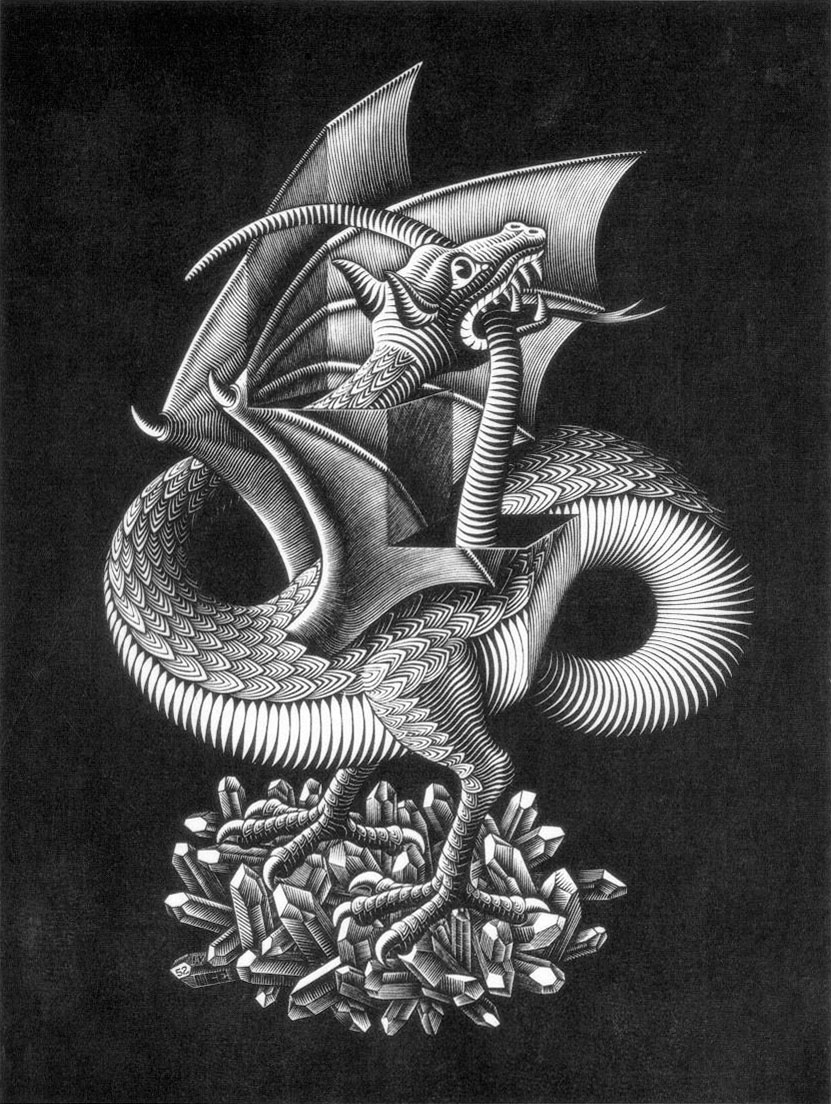
\includegraphics{img_076.jpg}
\caption[龙,艾舍尔作。]
  {龙,艾舍尔作(木刻,1952)}
\end{figure}

艾舍尔提供的一个形象画面对于支持这里的直观极有用处:那就是他的作品《龙》(\fig{76})。这幅画最突出的特点——自然也是它的主题——是一条咬着自己尾巴的龙。这里具有全部的哥德尔内涵。不过,这幅画还有更深一层的主题,艾舍尔本人曾写了下述很有意思的注释。第一条注释说的是他的一组素描,它们全与“平面和空间的冲突”有关,第二条注释是专门讲龙的。
\begin{quote}
\begin{enumerate}[wide,label=\Roman*.]
\item 我们所在的三维空间是我们所知道的唯一的现实世界,二维空间就像四维空间一样完全是虚构的,因为没有什么东西是平的,哪怕是磨得最光的镜子。不过,我们仍然认为一堵墙或一张纸是平面,而且——说起来也怪——就像人们自古以来所做的那样,我们仍将继续由于这种平的表面而对空间产生错觉。画上几条线,然后宣布:“这是房子。”这的确有点荒谬。这种奇特的情形就是下面五幅画\lnote{(包括《龙》在内)}的主题。\note{艾舍尔,《艾舍尔版画集》[\bn{The Graphic Work of M. C. Escher}],纽约;Meridian Press, 1967年版,第21页。}

\item 不管这条龙多么想变成空间的形象,它仍然是待在平面上。印着龙的这张纸上有两处切口,它们折起来露出了两个方孔。可这条龙是个顽强的家伙,它不顾自己的二维性,坚持认为它具有三维性,于是把头伸出其中一个孔,把尾巴伸出另外一个孔。\note{艾舍尔,《艾舍尔版画集》[\bn{The Graphic Work of M. C. Escher}],纽约;Meridian Press, 1967年版,第22页。}
\end{enumerate}
\end{quote}
这第二条注释很能说明问题。其要点是,不管你多么聪明地想在二维中模拟三维,总要遗漏某些“三维的本质”。这条龙极力想挣脱它的二维性,无视自己画在其上的那张纸是二维的,把头伸了出来。然而自始至终,我们站在画外却可以看到这完全是可悲而徒劳的。因为,龙也好,孔也好,折起来也好,统统不过是这些概念在二维空间中的模拟,没有一个是真的。然而龙却走不出它的二维空间,因而不能像我们一样知道这一点。事实上,我们还可以把艾舍尔的画里所表述的想法无限地做下去。例如,我们可以把它从书上撕下,叠起来,在上面剪个洞,再从洞里把它掏过来,为把这团东西变成二维的,我们再给它照相。对照片,我们还可以施用同样的手法。每一次,只要是最后又变到二维的——不论我们以为已经多么巧妙地在二维空间中模拟了三维空间——它就又得遭到切开,再叠起的厄运。

现在,借用艾舍尔的这个极好的隐喻,我们回过头来看看程序与人的对垒。我们谈过打算把“哥德尔算子”装进程序自身的事情。那好,即使我们已经写出了一个执行这一运算的程序,这个程序仍然抓不住哥德尔方法的实质。因为再一次地,我们在系统外面还能用它自己做不到的办法来“将死”它。可是,这样一来,我们还是在与卢卡斯辩论吗?还是在反对他吗?

\section{智能系统的限度}

是在反对。正是由于我们无法写出执行“哥德尔化”的程序这样一个事实,才使我们多少有点怀疑我们自己是不是真能在一切情形下都能运用哥德尔手法。抽象地论证“能做”哥德尔化是一回事,具体搞清在每种情形下究竟该如何做又是一回事。事实上,随着形式系统(或程序)的复杂性逐步升级,我们自己做哥德尔化的能力最终也会开始动摇。因为,如我们前面说过的,毕竟没有任何算法手段能描述如何去施行它。如果我们没有办法明确地说出在所有的情形下使用哥德尔方法会遇到些什么,那么对我们每个人来讲,最后都会碰到复杂得简直无法搞清该如何下手的情形。

自然,人的能力的这种分界线总有些说不清楚,就像一个人到底能从地上提起多重的东西这个界限一样。某一天你可能提不起$250$斤的东西,可另一天可能又提得起。不过不管怎么说,总不会有一天你能提起$250$吨重的东西。按照这样一种意义,尽管每个人哥德尔化的界限是模糊的,但对任何一个人,都存在一个系统是大大超出他的哥德尔化能力的。

在《生日大合唱哇哇哇乌阿乌阿乌阿……》中直观地说明过这种想法。一开始,看上去很明显,乌龟想要纠缠阿基里斯多久就能纠缠多久。而后来阿基里斯则试图一举概括全部答案。这是和前面做出的任何反应都截然不同的一招,从而得到一个新名字“$\omega$”。这个名字的新颖性十分重要。它是不得不超出老的命名方案——那只包括了全体自然数的名字——的第一个例子。此后就得到某些进一步的扩充,其中一些扩充的名字颇为淸楚,而另一些则相当玄妙。不过,我们最终再一次用光了名字,这时我们把这些答案模式
\[
\omega, \omega^\omega, \omega^{\omega^\omega},\dotsc
\]
全部集结为一个复杂得难以想象的答案模式。给它起个全新的名字,叫“$\varepsilon_0$”。之所以需要一个新名字,是因为采取了一类全新的步骤——遇到了某种不规则性。所以必须要提出一个特定的新名字。

\section{不存在给序数命名的递归规则}

现在,你可能会冒出一个想法:在从序数到序数(我们用“序数”指称那些无穷量的名字)这一进程中,那些不规则性可以由一个计算机程序来处理。也就是说,可以有一个程序按某种规则的方法来产生新的名字,而在它力不从心的时候,则乞灵于能提供新名字的“非规则性处理器”,然后再回到那个简单程序上。但这样还是不行。结果会是:这些不规则性本身也是按一种不规则的方式发生的。所以我们还得有一个二阶程序——也就是说,要有一个生产那些制造新名字的程序的程序。即使如此,也仍然不够,最终还得要一个三阶程序。如此下去,再如此下去。

这种也许看上去颇为荒唐的复杂性,完全出自阿朗佐·丘奇和斯蒂芬·克利尼关于这些“无穷序数”的结构的一条深刻的定理:

\begin{block}
不存在能给每个构造性序数命名的递归相关的标号系统。
\end{block}
什么是“递归相关的标号系统”,什么是“构造性序数”,我们只得留待技术性更强的资料——如哈特利·罗杰斯的著作——去解释。不过,直观的想法已经给出了。随着序数越来越大,就有不规则性和不规则性中的不规则性,以及不规则性中的不规则性中的不规则性,等等。任何一个方案,无论它多复杂,都不能给所有的这种序数命名。由此可知,没有一个算法型的方法能说清如何对所有种类的形式系统使用哥德尔方法。除非我们固执得不可理喻,我们只能承认任何一个人都必将在某一点上达到他自己作哥德尔化能力的极限。超过这一点之后,具有这种复杂性的形式系统尽管由于哥德尔的理由是不完全的,但却会和人一样强有力。

\section{对卢卡斯的其它反驳}

这不过是反驳卢卡斯立场的一种方法。还有一些方法可能更为有力,我们后面将会谈到。不过,这里的这个驳论特别会使人感兴趣,因为它提出了试图创造一个能够走出自身、完全从外部观察自己、并对自己使用哥德尔手段的计算机程序的想法。当然,这就像一台唱机能播放会导致自己崩溃的唱片一样,是不可能的。

不过,不应该因为这个理由而认为TNT有缺陷。如果什么地方出了毛病,也一定不是在TNT内,而是由于我们对它所能做的事情期望过高。此外,认清下面这一点是有好处的:我们同样很容易受到被哥德尔移植到数学形式主义中的文字圈套的打击:那就是说谎者悖论。这一点由怀特利巧妙地指了出来。他提出了一个句子:“卢卡斯不能前后一致地断定本句子。”如果你想一下这句话,那就会看出:\pnum{1}它是真的,以及\pnum{2}卢卡斯不能前后一致地断定它。所以,对于世界上的真理而言,卢卡斯也是不完全的。他大脑组织中反映世界的方法使他不能既是前后一致的,同时又能断定那个真句子。不过卢卡斯也并不比我们中的任何一个人更脆弱。他和一个老练的形式系统是一个数量级的。

搞清卢卡斯论证中的错误的一个有趣方法,是把它翻译成男人和女人之间的一场较量……从前有那么一天,思想家卢克思在游历的途中,碰见了一个不认识的东西——一个女人。这样的东西他以前从未见过。一开始,他由于她长的与自己很像而非常激动,但之后就有点害怕了。他冲着周围的男人们喊道:“瞧!我能看见她的脸,而这是她做不到的事——所以女人决不会和我一样!”这样,他就证明了男人比女人优越,变得轻松多了(而他的男同胞也都放下心来)。顺便插一句,同样的论述也能证明卢克思比其他所有的男人也都优越——可他并没有对他们指明这一点。那个女人转过身来争辩说:“对,你能看见我的脸,这我做不到——但我能看见你的脸,这件事你也做不到!我们打平手。”然而,卢克思却提出一个出人意料的反驳:“很遗憾,如果你以为你能‘看见’我的脸,那就错了。你们女人所做的事情与我们男人并不一样。正如我已经指出的,你们是低能的,因而不配用同一个名称。你可以称之为‘妇见’。你能‘妇见’我的脸,这并不说明问题,因为情况并不对称。懂了吗?”“我妇懂了”,那个女人“妇答”道,然后就“妇走”了……

是的,这是一种鸵鸟式的论点。可你要是也确信在这场智力竞赛中男人们和女人们永远跑在计算机前面,那你就不得不这样看问题。

\section{超越自我——一个现代的神话}

仔细想一想我们人类是否能跳出自身——或者是,计算机程序是否能跳出自身——仍是极为引人入胜的。当然,程序有可能自己修改自己——不过这种可修改性必须首先是该程序中固有的部分,所以不能算做“跳出系统”的例子。不论一个程序怎样迂回曲折地来到自己外面,它仍然遵循自身的固有规则。对程序来说,逃脱的可能性并不比一个活人决计不服从物理定律的可能性更大。物理定律是个强制系统,什么也逃不掉。然而一个不那么宏大的抱负是可能实现的,那就是:一个人当然可以从他的大脑的一个子系统跳到一个更宽广的子系统中去。我们偶尔也能打破常规。不过这仍然属于人的大脑中各个子系统之间的相互作用,只不过会觉得它很像是完全走出了自身。与此类似,完全可以想象把部分“走出自身”的能力嵌入一个计算机程序。

无论如何,弄清楚“感知自身”和“超越自身”之间的区别是很重要的。你可以用各种各样的方法来看到自己——用镜子、用照片或电影、用录像带、靠别人的描绘、采用精神分析法等等,但你决不可能冲破皮肤站到自己外面来(这里不谈那些现代神秘运动和流行的“超心理学”流派)。TNT能够谈论自身,但不能跳出自身。一个计算机程序可以修改自己,但不能违背自身的指令——充其量也只能通过服从自身的指令来改变自己的某些部分。这倒使人想起一个幽默的悖论问题:“上帝能不能造出一块他自己举不动的石头?”

\section{广告和框架手法}

这种跳出系统的愿望到处可见。在艺术、音乐及人类其它事业的发展过程中,都有它的踪迹。就连制作广播电视广告这类不足称道的行业里,也有它的存在。欧文·高夫曼在他的著作《框架分析》中出色地领悟和描绘了这种潜在的趋向:

\begin{quote}
例如,一位著名的专业演员做完了一个广告,摄影机还在对着他,他就明显地做出解除了任务的样子,沉浸于享用他刚刚宣传的那种产品的实际快乐之中。

当然,这只是在制作电视和广播广告时利用框架手法的一个例子。这种表面上的自然而然能克服(他们这么希望)观众中蔓延着的冷漠性。于是就常常会有儿童的声音,以期造成一种似乎是未经训练印象;利用街上的噪音和其他一些效果,以期造成被访问者并不领取酬金的印象;错了的开始、不时停顿、插科打浑、以及重叠的话语,给人造成现场谈话的假象;另外,按维勒斯的方法:打断一个企业单调重复的广告而报告该企业推出新产品的消息,偶尔也插入公众所感兴趣的简短通讯。这种作法似乎可以保持现代观众的信任。

观众越是退而把一些次要的细节当作检验标准,广告商就追得越紧。结果就是一种相互污染,一种杂乱无章。这种现象同时也在被政治家的公共关系顾问以及微观社会学传播着\lnote{(后者稍好一些)}。\note{高夫曼,《框架分析》,第475页。}
\end{quote}
这样,我们又有了另一个逐步升级的“龟蟹之战”的例子——这次是事实和广告对垒。

\section{辛普利奇奥、萨尔维亚蒂、萨哲杜:\\为什么要三个?}

跳出系统的问题与追求完全的客观性之间,有一个引人入胜的联系。我在读尧奇的《量子是实在的吗?》中的四段对话(基于伽利略的四段《关于两种新科学的对话》)的时候,发现自己搞不清为什么要有三个角色出场:辛普利奇奥、萨尔维亚蒂和萨哲杜。只有辛普利奇奥这位受过教育的傻瓜和萨尔维亚蒂这位学识渊博的思想家两个人为什么就不行呢?萨哲杜有什么用处?是的,他被当作中立的第三派,不偏不倚地掂量两边的份量,作出“公平的”、“无偏见的”裁决。看起来很公正,可还有一个问题:萨哲杜总是赞成萨尔维亚蒂而从不赞成辛普利奇奥。人格化的客观性怎么变成了人的好恶了呢?当然,一种答案就是:萨尔维亚蒂在阐述正确观点,所以萨哲杜没有选择的余地。可是,公平性和“机会均等”又在哪儿呢?

由于增加了萨哲杜,伽利略(以及尧奇)就把牌洗得对辛普利奇奥多一些不利,而不是少一些。也许需要增加一个更高层次的萨哲杜——他对整个环境都是客观的……你可以看到这会导致什么。我们将得到一个“客观性逐步升级”的无终点序列,它有着“决不会比第一层更客观”这样一个吸引人的性质:在第一层上,萨尔维亚蒂就是对的,而辛普利奇奥是错的。所以,疑难点仍在于:为什么增加萨哲杜?答案是:就某种直观感染力而言,这种做法造成了走出该系统的错觉。

\section{禅宗和“走出”}

在禅宗里,我们也能看到这种对超出系统的概念的神往。例如那个洞山告诉弟子们“佛性上人是非佛”的公案。也许,超越自我乃是禅宗的中心主题。禅宗门人总是企图更深刻地了解他自己是怎么回事,靠的就是逐步走出他所看到的自己,并打破那些他领悟到是在束缚自己的清规戒律——当然,也包括禅宗本身的那些清规戒律。沿着这条难以捉摸的路线下去,也许到某一处就顿悟了。在任何情形(如我见到的那样),希望都在于:通过逐步加深一个人的自我意识,逐渐扩展“该系统”的范围,他最终将会感到与整个宇宙相一致。
